\chapter{ExxonMobil Model}
\label{ch:exxonmobilmodel}

\section{Introduction}
The model is being developed by ExxonMobil, originally beginning in 2021.  It is an axial-torsional system designed to model the dynamics of drill strings while drilling and tripping. It can be used in both vertical and inclined wells under various operational conditions.  BHA components such as drill pipes, HWDP, drill collars, and mud-motors can be incorporated.  Additional features include bit-rock interaction and incorporation of heave compensator dynamics. Validation of the model was done by comparing simulation results with field data from rotational startups, off-bottom rotations, and post-connection operations.

\section{Model Description}
The model employs a 2 DOF per node, axial-torsional system and uses a lumped-parameter technique (\referencename~\cite{ref:dixit2021a}). The axial and torsional DOF are coupled through the friction terms and the bit-rock interaction.  There is not a coupling from material properties, the inertia terms, et cetera.  The governing equations of motion are solved by a fourth and fifth order Runge-Kutta-Fehlberg (RKF) method (\referencename~\cite{ref:shor2022a}).  This is a popular solver that has been implemented many times, including as the well known Matlab \textcode{ODE45} function. Assumptions of the model are:
\begin{bulletedlist}
	\item A simplified bit model (see \sectionname~\ref{sec:exxonbitmodel})
	\item No lateral motion
    \item No lateral bending moments (soft string model)
    \item The entire drill string is in contact with the wellbore (soft string model)
	\item The effects of cuttings distribution on the friction is homogeneous
	\item Viscous damping is included
	\item Cased and open hole sections have the same friction factors
    \item Friction between the drill string and wellbore is modeled as a type of Stribeck friction (see \sectionname~\ref{sec:exxonfrictionmodel})
    \item Tool joints effects can be included
\end{bulletedlist}
%Drilling fluid damping is uniformly applied throughout the system.

The bit-rock interaction model is based on depth-of-cut and calculated by tracking the bit-depth relative to hole-depth. At each time step, the bit is considered to be drilling ahead when the DOC is higher than zero (the bit depth is greater than the hole depth) and the angular displacement of the bit is in the direction of the input rotation (i.e., the bit is not standing still or rotating backwards).  This feature contributes to a more realistic representation of the drilling process.

The Python-based source code is designed using a modular approach.  Most functions are distributed across separate Python files and are easily accessible by importing them. The code's operational instructions and guidelines are included in a manual (\referencename~\cite{ref:dixit2021a}), offering users guidance on running the code effectively.

\subsection{Top Drive Model}
The model utilizes the axial and rotational velocity of the top-drive as input. These are integrated to calculate the corresponding axial and rotational displacements of the top-drive.

Torque on top-drive can be derived as
\begin{equation}\label{TorqueEQ}
  \tau_{td} = k_{t1} \theta_{td}
\end{equation}
where $\tau_{td}$ is top-drive torque, $k_{t1}$ is torsional stiffness of first drill-string element, and $\theta_{td}$ is top-drive rotation angle. \reviewcomment{This equation and explanation still seems off.}

The model incorporates an additional parameter known as \emph{heave} which accounts for the influence of waves during offshore operations. Additional computations are conducted to determine heave displacement and the effect on the rate of penetration (ROP). These calculated values are subsequently added to the original top-drive ROP and displacement data. The heave ROP and displacement calculations are represented by the equations
\begin{equation}\label{Z_heave}
  Z_{heave} = x \cdot \sin(\omega \cdot (t - t_{heave\_delay}))
\end{equation}
\begin{equation}\label{ROP_heave}
  ROP_{heave} = x \cdot \omega \cdot \cos(\omega \cdot (t - t_{heave\_delay}))
\end{equation}
where $Z_{heave}$ is the displacement, $ROP_{heave}$ is heave ROP, $x$ is heave amplitude, $\omega$ is heave angular velocity, $t$ is time, and $t_{heave\_delay}$ is heave delay time.

\subsection{Bit Model}
\label{sec:exxonbitmodel}
The laws governing the bit-rock interface in drilling operations primarily rely on the relationships between weight on bit, torque on bit, rate of penetration, and angular velocity. These interdependent variables play a crucial role in achieving efficient drilling while also influencing the emergence of drilling dysfunctions within the system. The forces and torque exerted on the bit are directly influenced by the instantaneous changes in axial and angular velocities.

The interaction between PDC bits and the rock formation encompasses a combination of cutting and frictional contact, as identified by \referencename~\cite{ref:detournay1992a}.   This is modeled by decomposing the weight on bit and torque on bit into cutting and frictional components, which are contingent upon the strength of the rock formation being drilled.  The WOB and TOB are given as
\begin{equation}\label{WOB}
  WOB_{bit} = (k_{WOB} DOC_{iteration}) + (c_{bit-axial} \dot{Z}_{bit-ietration})
\end{equation}
\begin{equation}\label{Torque}
  TQ_{bit} = k_{TQ} DOC_{iteration\; array} (\pm1)
\end{equation}
where $k_{WOB}$ is the weight on bit coefficent, $k_{TQ}$ is the torque on bit coefficient, $DOC_{iteration}$ is depth of cut at the current time step, $c_{bit-axial}$ is axial viscous damping, and $Z$ is bit displacement.  The rock strength is incorporated into the coefficients $k_{WOB}$ and $k_{TQ}$.  The dependency on the depth of cut represents the material removed during drilling.

\subsection{Friction Model}
\label{sec:exxonfrictionmodel}
A Stribeck type friction model is used for the static and dynamic friction (\referencename~\cite{ref:cayeux2020a}).  The model takes into account the velocity, well trajectory, and buoyancy effects when calculating the friction forces. The friction model also has the following features:
\begin{bulletedlist}
    \item Friction model is coupled, the resultant velocity of the axial and torsional DOF are use to determine the friction force
    \item No movement occurs until the resultant (combined axial and torsional) reaction force reaches static limit
\end{bulletedlist}

The Stribeck model is used to avoid the discontinuities when $\vec{v}_s$ tends to zero that occur with the Coulomb model (the jump from static to dynamic friction coefficients). The following \equationname~\ref{Stribeck velocity} was proposed by Tunstin (\cite{ref:tustin1947a}).
\begin{equation}
	\label{Stribeck velocity}
	\mu_{eff} = \mu_{d} + (\mu_{s} - \mu_{d}) e^{-(|V_s|/V_{CS})}
\end{equation}
where $\mu_{eff}$ is effective friction factor, $V_{CS}$ is Stribeck critical velocity, $\mu_{s}$, and $\mu_{d}$ are the static and dynamic friction factors, respectively.


\begin{figure}
	\begin{minipage}[t]{\linewidth}
		\begin{minipage}[t]{0.32\linewidth}
			\centering
			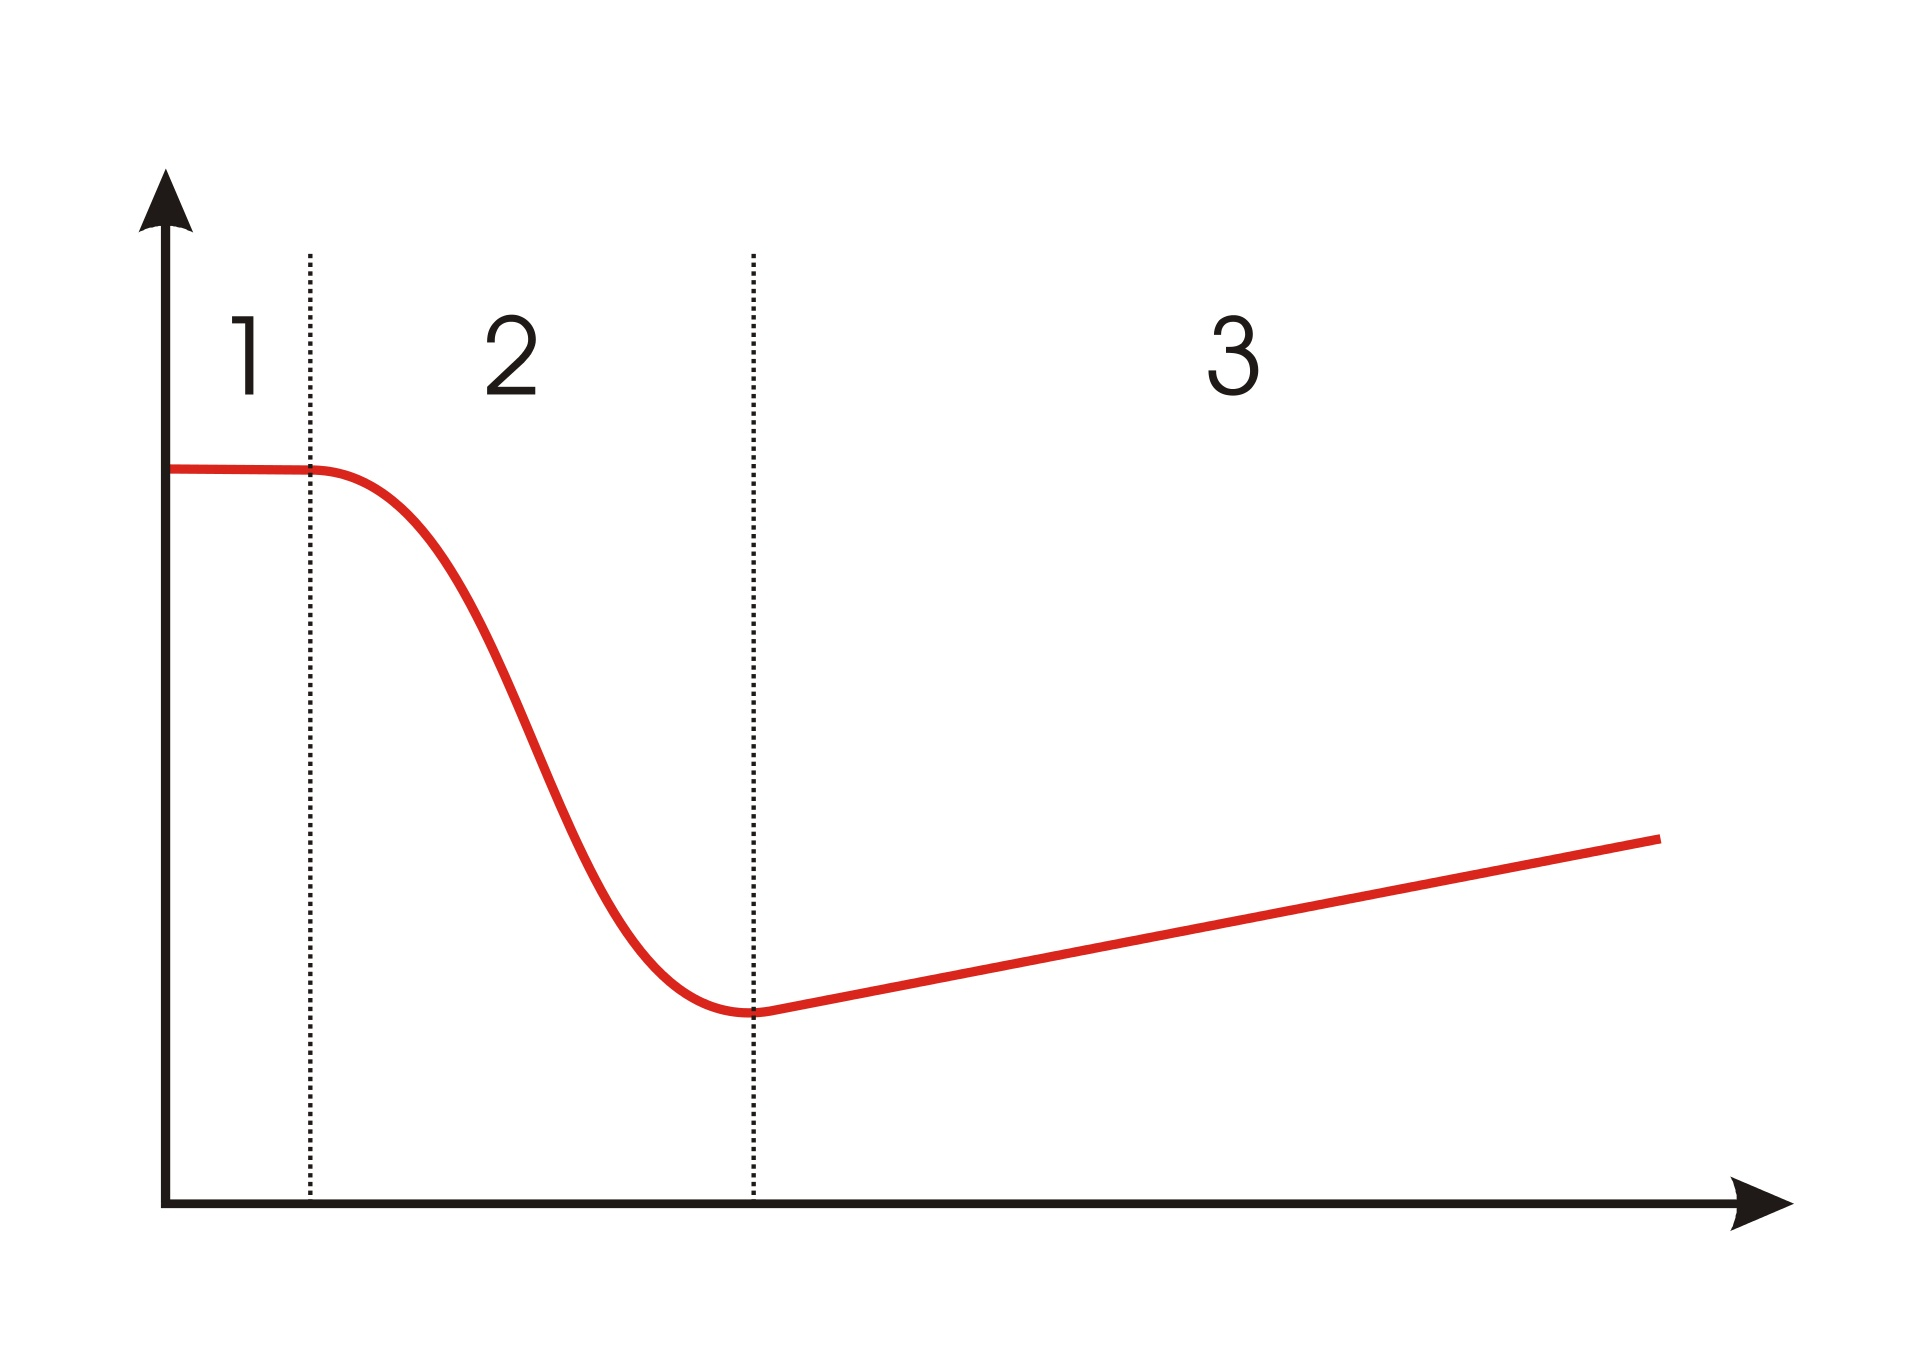
\includegraphics[width=\linewidth]{schematicstribeckcurve}
			\subcaption{Schematic Stribeck curve (Hersey number on horizontal axis, friction coefficient on vertical) 1 Boundary lubrication, 2 Mixed lubrication, 3 Hydrodynamic lubrication.}
			\label{fig:schematicstribeckcurve}
		\end{minipage}
		\hfill
		\begin{minipage}[t]{0.32\linewidth}
			\centering
			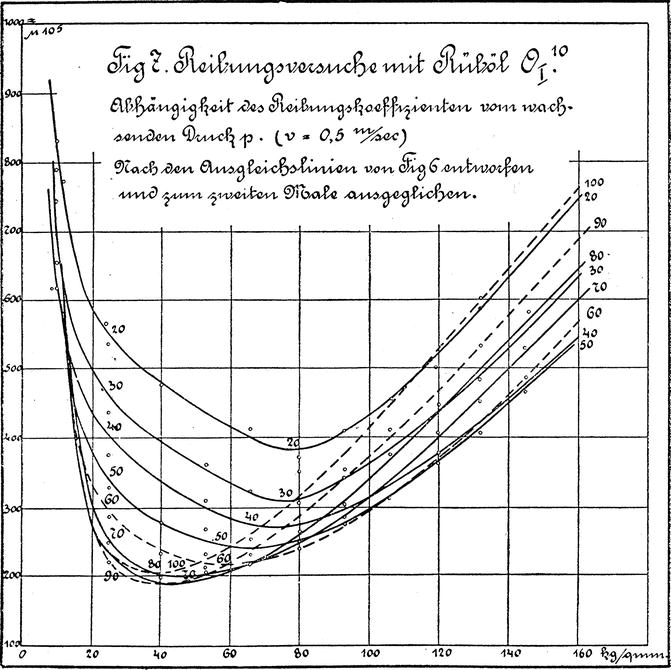
\includegraphics[width=\linewidth]{Martens_curves}
			\subcaption{Typical Stribeck curves obtained by Adolf Martens.}
			\label{fig:stribeckcurvesbymartens}
		\end{minipage}
		\hfill
		\begin{minipage}[t]{0.32\linewidth}
			\centering
			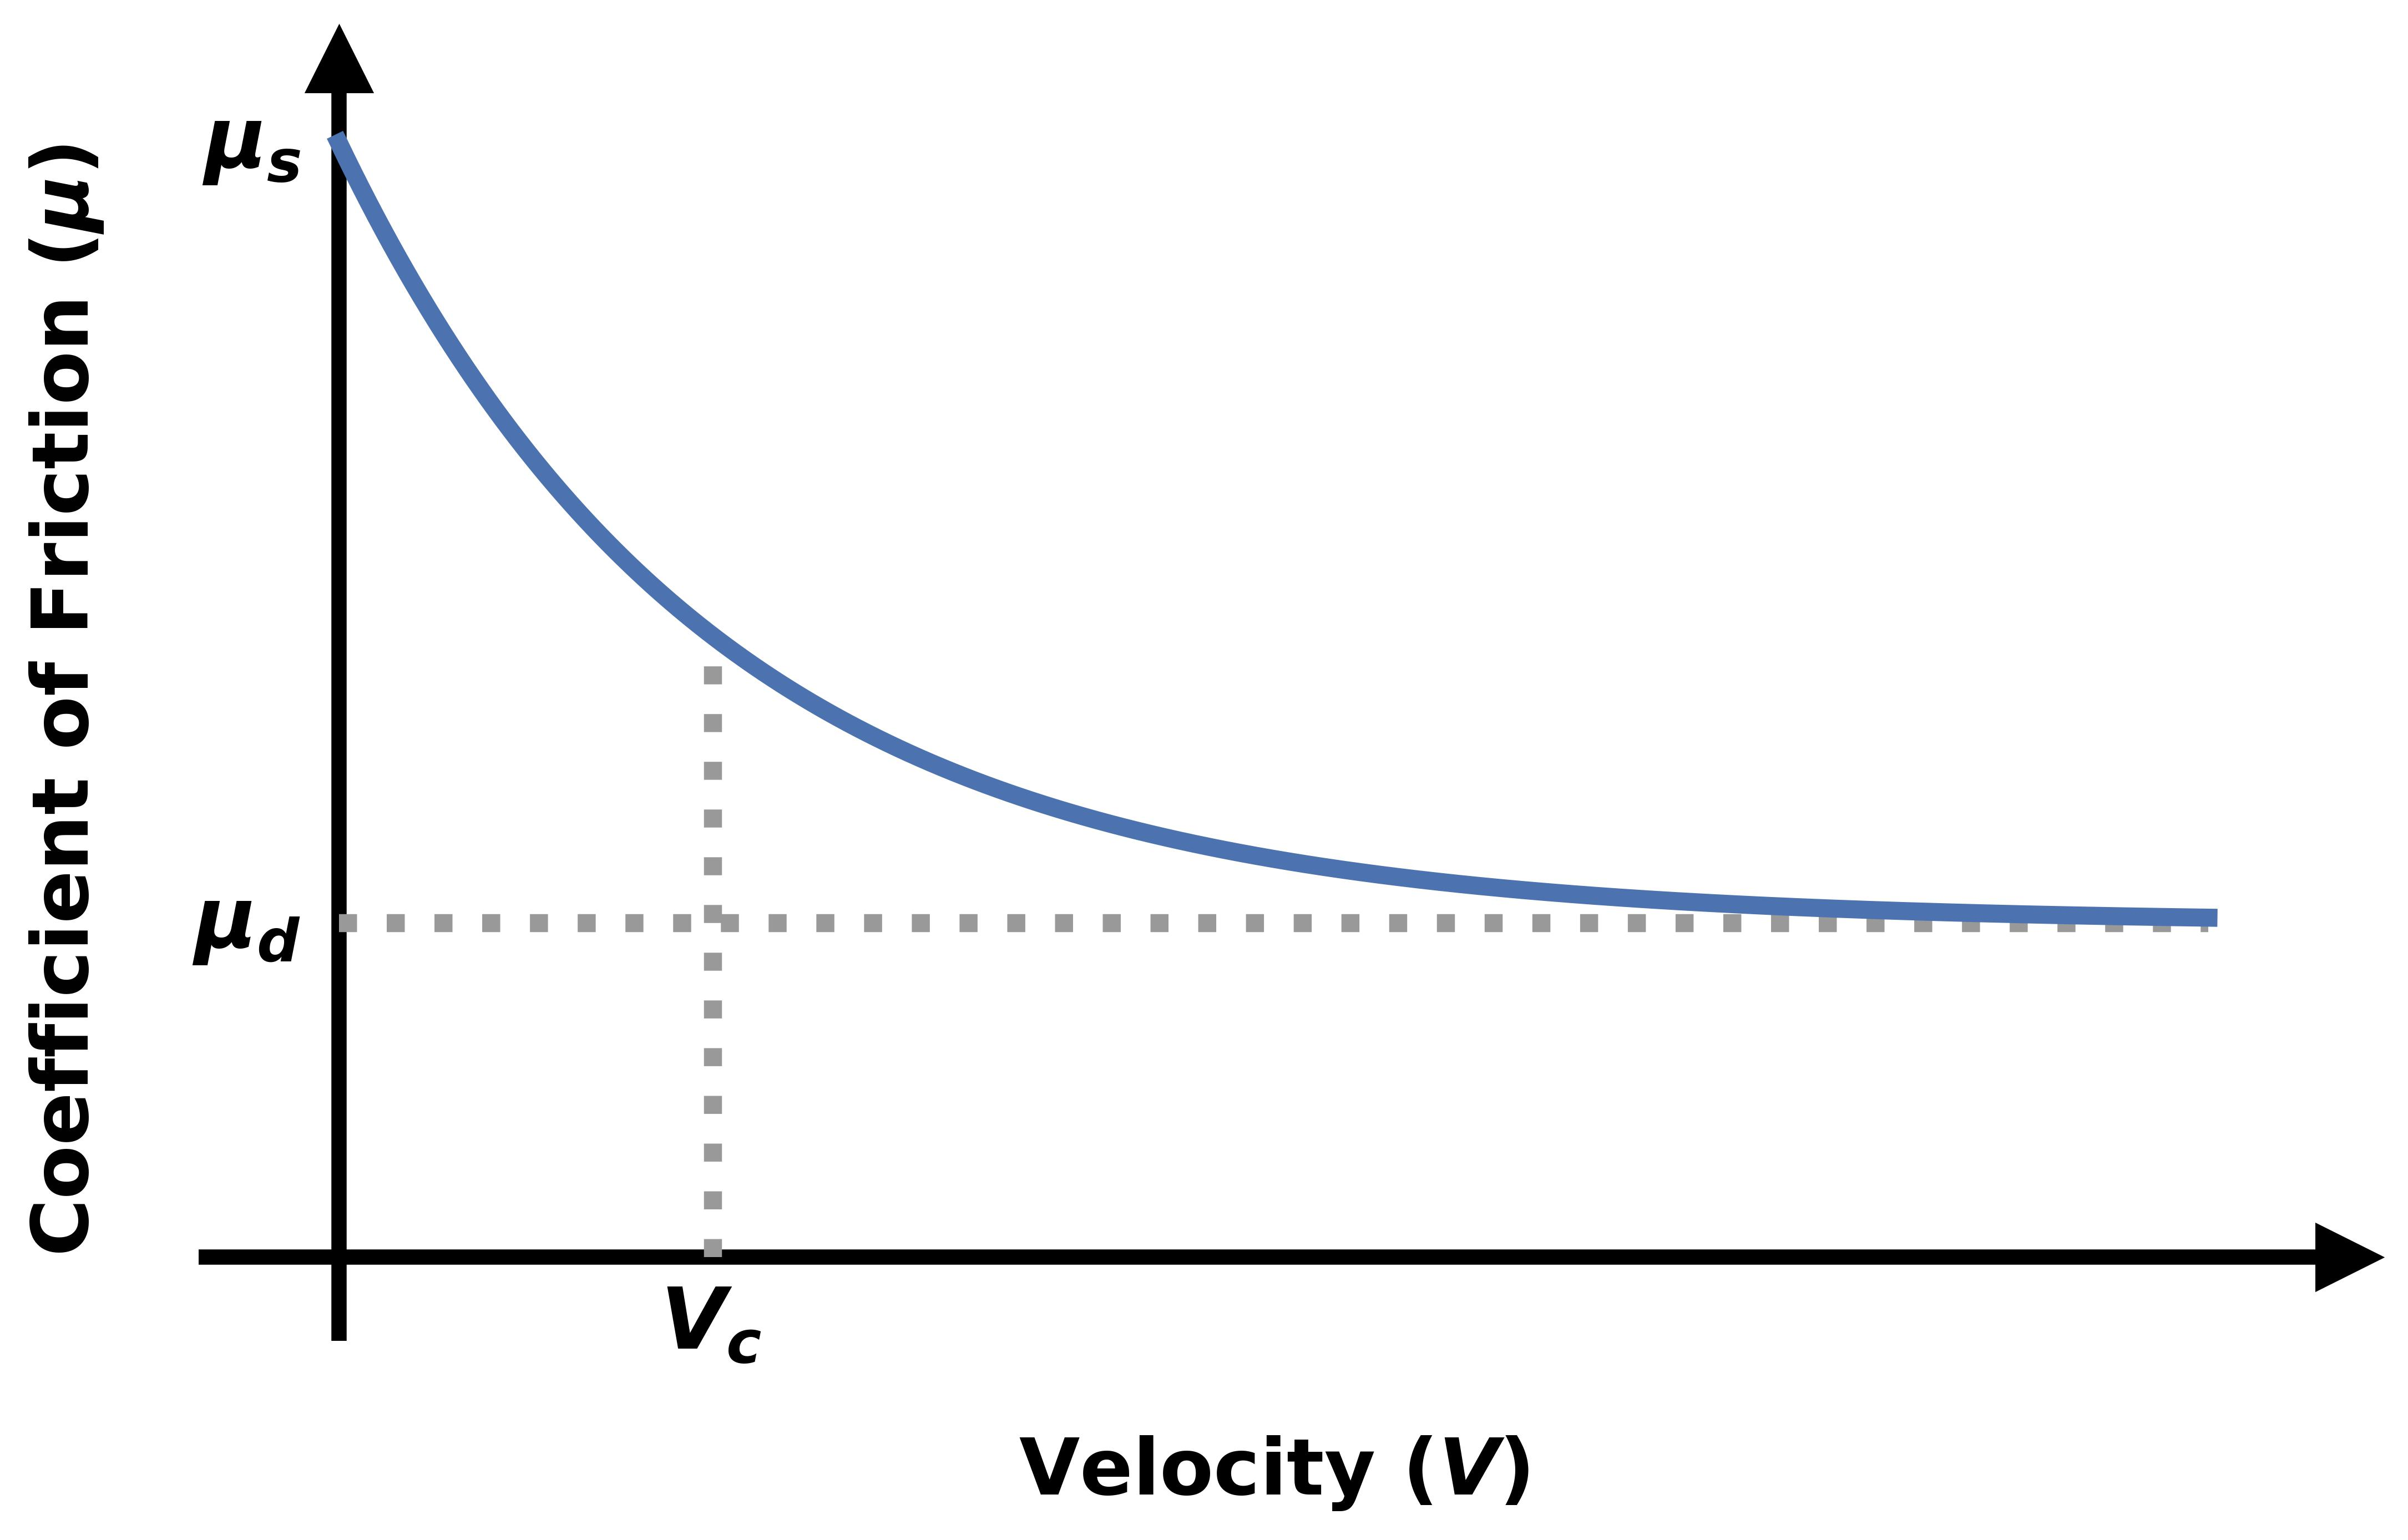
\includegraphics[width=\linewidth]{stribeckfrictioncurve}
			\caption[Stribeck friction model]{An example of a Stribeck friction model with .}
			\label{fig:stribeckfrictioncurveexample}
		\end{minipage}
	\end{minipage}
	\caption[Examples of Stribeck friction curves]{Examples of Stribeck friction curves.  (from \referencename~\cite{ref:martens2023a})}
	\label{fig:stribeckfrictioncurve}
\end{figure}
which is shown in \figurename~\ref{fig:stribeckfrictioncurve}


The friction is combined with viscous damping (in a manner similar to the source term in the A-S model) \reviewcomment{Is this true, or is there a Stribeck friction model that a velocity dependence in the dynamic friction region and a separate viscous damping term?} to create the curve shown in \figurename~\ref{fig:exxonmobilfriction}.
\begin{figure}
	\centering
	\includegraphics[width=\linewidth]{exxonmobilfriction}
	\caption[Comparison of friction models]{The combined friction and viscous damping model presented in \referencename~\cite{ref:dixit2021a}}
	\label{fig:exxonmobilfriction}
\end{figure}

The dynamic friction force\footnote{This is a conceptualization of the calculation. The presentation in the reference documents and implementation in the code is slightly different.} is calculated as
\begin{equation}\label{dynamic_force}
  \mbf{F}_{\mu,k} = - \mu_{eff} F_{n} \frac{\mbf{V}_{s}}{\|\mbf{V}_{s}\|}
\end{equation}
where $\mbf{F}_{\mu,k}$ is the dynamic friction force vector (axial and torsional), $\mu_k$ is the dynamic friction factor, $F_n$ is the scalar normal force, and $\mbf{V}_{s}$ is the velocity vector.\footnote{In the reference material, $\mbf{V}_{s}$ is a scalar value called $V_{sliding}$. $V_{sliding}$ is the magnitude of the combined axial and torsion velocity of the drill pipe at the OD of the drill pipe where it contacts the wellbore wall.  The authors have not used the term ``sliding'' in order to prevent any confusion with the ``sliding'' mode in drilling used to build curves.  The drilling sliding mode may imply an axial only displacement, which is not the case for the friction calculation.} The dynamic friction force opposes the direction of motion (\equationname~\ref{dynamic_force}).

The static friction force acts in the opposite direction of the sum of all tangential forces when there is no motion ($V_{Sliding}=0$).  That is,
\begin{equation}\label{zero}
  F_{\mu,s} + \sum F_{Ext} = 0
\end{equation}
where $F_{\mu,s}$ is static friction force and $\sum F_{Ext}$ is the sum of external forces.

%The friction is modeled as Stribeck friction.  The static friction applies when there is no slip ($\|\mbf{V}_{s}\|$=0), where the velocity vector, $\mbf{V}_{s}$, is a function of rotational and axial velocities of the pipe.
%
%More details for the velocity vector can be seen from (\referencename~ \cite{ref:cayeux2018a}). The magnitude and direction of the static friction force are equal and opposite to that of the external force at contact point, respectively (\equationname~\ref{eq:exxon_staticFF}). However, once the external foce exceeds the limit of static friction, $\mu_s \vec{F_n}$, where $\mu_s$ is static friction factor and $\vec{F_n}$ is normal force at dril string - wellbore contact, the drill string starts to slide ($\vec{v}_s > 0$) and dynamic friction is applied. The dynamic friction acts in the opposite direction to the velocity vector. The equation of dynamic friction force is shown in \equationname~\ref{eq:exxon_dynamicFF}, where $\mu_k$ is dynamic friction factor.
%\begin{equation}
%	\label{eq:exxon_staticFF}
%	F_{\mu,s} + \sum F_{Ext} = 0
%\end{equation}
%\begin{equation}
%	\label{eq:exxon_dynamicFF}
%	\vec{F_{\mu, d}} = -\mu_d ||{\vec{F_n}}||\frac{\vec{v}_s}{{||\vec{v}_s}||}
%\end{equation}




The total damping applied in the system is a linear combination of the friction and viscous damping. \figurename~\ref{figure_Exxon_friction} illustrates the Stribeck friction and total friction as a function of sliding velocity.
\begin{figure}
	\centering
	\includegraphics[width=6.5in]{Exxon_friction}
    \caption[Friction model for ExxonMobil model]{Friction model for ExxonMobil model. Left and right figures are friction models in ExxonMobil model only when Stribeck friction is considered and both Stribeck and viscous friction are included, respectively. Stribeck friction refers to the friction from drill string and wellbore contact. $F_{\mu, s}$ is static friction, $C$ is viscous friction coefficient (same as viscous damping) and $V_{CS}$ is Stribeck critical sliding velocity. Total friction in the system is the linear combination between Stribeck and viscous friction. \reviewcomment{Aren't this just two forms of Stribeck friction?}}\label{figure_Exxon_friction}
\end{figure}

%Furthermore, the order of the viscous damping constants is maintained consistently to ensure that the system remains in an ideal damp state, aligning with the field data. Values of viscous dampers are held constants during simulation, but the viscous frictional force will vary depending on the sliding velocities as can be seen in \figurename~\ref{fig:exxonmobilfriction}.

%Below, the friction model input parameters are listed.
%\begin{bulletedlist}
%    \item Equivalent diameter of pipe
%    \item Coulomb friction force
%    \item Coulomb friction force axial component
%    \item Coulomb friction force tangential component
%    \item Coulomb friction torque tangential component
%    \item Viscous friction force axial component
%    \item Viscous friction force tangential direction component
%    \item Axial and tangential components of net frictional force and torque
%\end{bulletedlist}

\section{Mathematical Background}

The set of partial differential equations that describe the motion of the drill-string can be combined into a coupled axial-torsional system of second-order differential equations.

\begin{align}\label{Governing equations}
     m_{i}\dfrac{\partial^{2}s_{i}}{\partial t^{2}} & = -k_{a,i}(s_{i}-s_{i-1}-l_{i}) + k_{a,j+1}(s_{i+1}-s_{i}-l_{i+1}) + \sum{F_{ext, i}} \\
     I_{i}l_{i}\dfrac{\partial^{2}\theta_{i}}{\partial t^{2}} & = -k_{t,i}(\theta_{i}-\theta_{i-1}-l_{i}) + k_{t,j+1}(\theta_{i}-\theta_{i+1}) + \sum{\tau_{ext,/ i}}
\end{align}

To convert these equation sets into vector form, we can represent the variables and their derivatives as vectors.

\begin{align}
  \{M\} \ddot{\boldsymbol{Z}}+\left\{C_a\right\} \dot{\boldsymbol{Z}}+\left\{K_a\right\} \boldsymbol{Z}+\boldsymbol{f}_{\text{fric}} &= \boldsymbol{F}_{\text{forcing}} \label{eq:em_axial_vector_form}\\
  \{J\} \ddot{\boldsymbol{\theta}}+\left\{C_t\right\} \dot{\boldsymbol{\theta}}+\left\{K_t\right\} \boldsymbol{\theta}+\boldsymbol{\tau}_{\text{fric}} &= \boldsymbol{\tau}_{\text{forcing}} \label{eq:em_torsional_vector_form}
\end{align}


\begin{align}
	\{M\} &= \left[\begin{array}{ccc}
				m_1 & \cdots & \vdots \\
				\vdots & \ddots & \vdots \\
				\vdots & \cdots & m_n
				\end{array}\right] \\
	\{J\} &= \left[\begin{array}{ccc}
			J_1 & \cdots & \vdots \\
			\vdots & \ddots & \vdots \\
			\vdots & \cdots & J_n  \\
  			\end{array}\right] \\
	\left\{C_a\right\} &= \left[\begin{array}{ccc}
							c_{a 1} & \cdots & \vdots \\
							\vdots & \ddots & \vdots \\
							\vdots & \cdots & c_{a n}
							\end{array}\right] \\
	\left\{C_t\right\} &= \left[\begin{array}{ccc}
							c_{t 1} & \cdots & \vdots \\
							\vdots & \ddots & \vdots \\
							\vdots & \cdots & c_{t n}
							\end{array}\right] \\
 	\left\{K_a\right\} &= \left[\begin{array}{ccc}
							k_{a 1} & -k_{a 2} & \cdots \\
							-k_{a 2} & \ddots & \vdots \\
							\vdots & \cdots & k_{a(n-1)}+k_{a n}
							\end{array}\right] \\
	\left\{K_t\right\} &= \left[\begin{array}{ccc}
							k_{t 1} & -k_{t 1} & \cdots \\
							-k_{t 1} & \ddots & \vdots \\
							\vdots & \cdots & k_{t(n-1)}+k_{t n}
							\end{array}\right] \\
  	F_{\text{forcing}} &= \left[\begin{array}{c}
							\boldsymbol{k}_{a 1} \cdot Z_{td} \\
							\vdots \\
							-\boldsymbol{k}_{a\_bit} \cdot \text{DOC}
							\end{array}\right] \\
	\mathcal{T}_{\text{forcing}} &= \left[\begin{array}{c}
							\boldsymbol{k}_{t 1} \cdot \theta_{td} \\
							\vdots \\
							-\boldsymbol{k}_{t\_bit} \cdot \text{DOC}
							\end{array}\right]
	\label{eq:emmatrixform}
\end{align}


\begin{mathwhere}[1.0in]
\mathdefitem{Z_0}{$\int V_0\ dt$;}
\mathdefitem{m_n}{drill string element mass;}
\mathdefitem{Z}{position (downward direction considered as positive);}
\mathdefitem{k_a}{axial stiffness of drill-string element;}
\mathdefitem{V_o}{top-drive (draw-works) axial velocity as input;}
\mathdefitem{Z_{td}}{top-drive (draw-works) axial displacement as input;}
\mathdefitem{\dot{Z}}{bit axial velocity (downward direction considered as positive);}
\mathdefitem{WOB_{surface}}{surface/top-drive WOB (in ROP control mode);}
\mathdefitem{J_n}{mass moment of inertia of drill string element;}
\mathdefitem{\theta}{rotation angle (clockwise direction is considered as positive);}
\mathdefitem{\omega_o}{top drive angular velocity as input;}
\mathdefitem{\theta_{td}}{top drive rotation as input;}
\mathdefitem{k_t}{torsional stiffness of drill-string;}
\mathdefitem{\dot{\theta}}{bit rotary velocity (clockwise direction considered as positive);}
\mathdefitem{TQ_{surface}}{surface/top-drive torque;}
\mathdefitem{{f}_{\text{fric}}}{Stribeck friction force;}
\mathdefitem{{\tau}_{\text {fric }}}{Stribeck friction torque.}
\end{mathwhere}

The differential equation sets are solved using the RKF solver. This solver was chosen for its efficiency in computational calculations.


\section{On-Bottom Example}
One of the features of this model is simulation of ``on-bottom'' case for drilling.  The Test Cases in this document are for the off-bottom case, so this feature was not directly compared.  However, it is an important feature that should be explored further. \figurename~\ref{findings} illustrates a comparison of an off-bottom and an on-bottom case.
\begin{figure}
  \centering
  \includegraphics[width=\linewidth]{comp_on_bottom}
  \caption[Comparison of off-bottom and on-bottom simulations]{Comparison of off-bottom (left) and on-bottom (right) simulations.  At 30 seconds, the bit touches bottom for the on-bottom case.  The expected results of increased torque, weight, depth of cut, et cetera are seen.}\label{findings}
\end{figure} 